\documentclass[12pt]{article}
\usepackage[margin=1in]{geometry} 
\usepackage{amsmath}
\usepackage{tcolorbox}
\usepackage{amssymb}
\usepackage{amsthm}
\usepackage{lastpage}
\usepackage{fancyhdr}
\usepackage{accents}
\pagestyle{fancy}
\setlength{\headheight}{40pt}


\newenvironment{solution}
  {\renewcommand\qedsymbol{$\blacksquare$}
  \begin{proof}[Solution]}
  {\end{proof}}
\renewcommand\qedsymbol{$\blacksquare$}

\newcommand{\ubar}[1]{\underaccent{\bar}{#1}}

\begin{document}

% Cover Page
\begin{titlepage}
  \centering
  
  {\scshape\LARGE University of British Columbia \par}
  \vspace{1cm}
  {\scshape\Large CPSC 425: Computer Vision\par}
  \vspace{1.5cm}
  {\huge\bfseries Assignment 5\par}
  \vspace{2cm}
  {\Large\itshape Simon Ghyselincks\par}
  \vfill
  Self-Studied based off of UBC CPSC 425 2023T1 course material\par

  \vfill

  % Bottom of the page
  {\large 2023\par}
\end{titlepage}

\lhead{UBC CPSC 425 Computer Vision: Assignment 5} 
\rhead{Term I 2023} 
\cfoot{\thepage\ of \pageref{LastPage}}

Based off of UBC CPSC 425 2023W T1 course material found at \texttt{https://mattabrown.github.io/425/assignments/Assignment5.html}

The goal is to explore image classification using some of the cutting edge techniques from 15+ years ago, namely bag of words and SVM. The images have a set of feature points and 128D SIFT descriptors. The descriptors are clustered using k-means to form a dictionary of words. These are basically textons that havd similarity and can be used to classify images. 

The test images can be classified by applying sorting each of the descriptors into the matching k-means cluster from the training set. 

To give a single descriptor vector to each image, we can use a histogram of the number of descriptors that match each cluster. This is a bag of words representation, where each cluster is a word and the image is a bag of words that has removed spatial information when it comes to the location of the feature points.

We inspect the average histogram for each of the 15 categories of images when it comes to the training set to get an idea of which images have a similar signature with this method. For this task only 60 cluster centers were used because it is very hard to visualize with a higher word count.


\begin{center}
  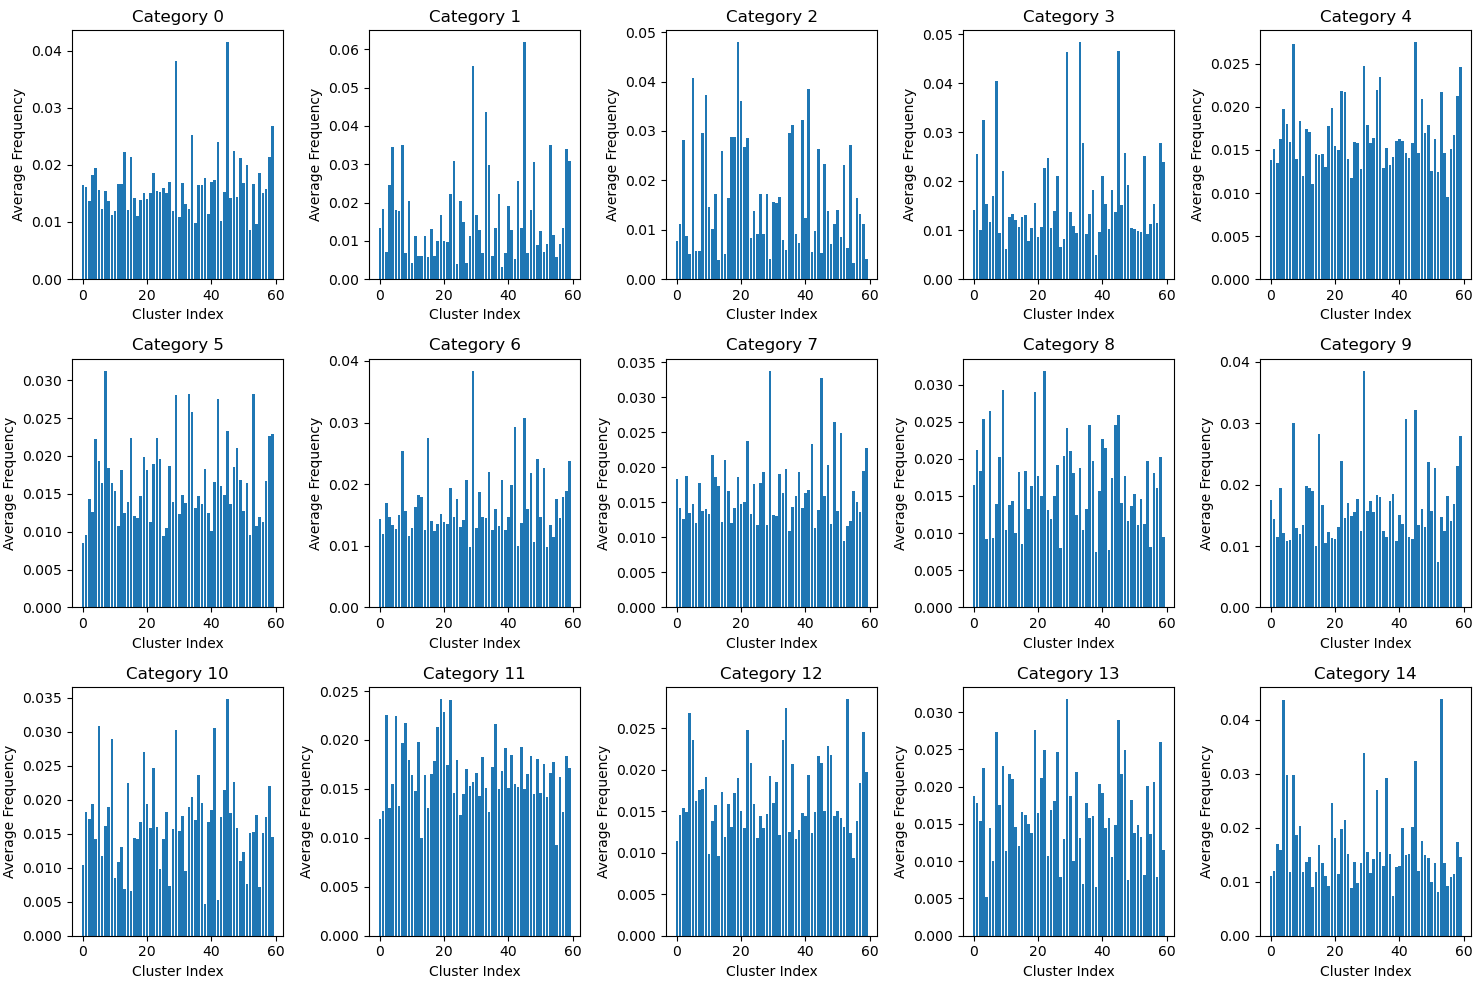
\includegraphics[width=1.05\textwidth]{imgs/histograms.png}
\end{center}

12-5 look similar and 12-4 as well. This is bassed on an overall shaper of the histogram.

\subsection*{Choosing K for KNN}
Too low of a value at $k=1$ overfits to the training data giving around 35\% accuracy. Too high of a $k$ when it reaches around 30 will also start to diminish the accuracy because of too much generalization. A good value is around $k=15$, giving close to $40\%$ accuracy.

The confusion matrix is as follows:

\begin{center}
  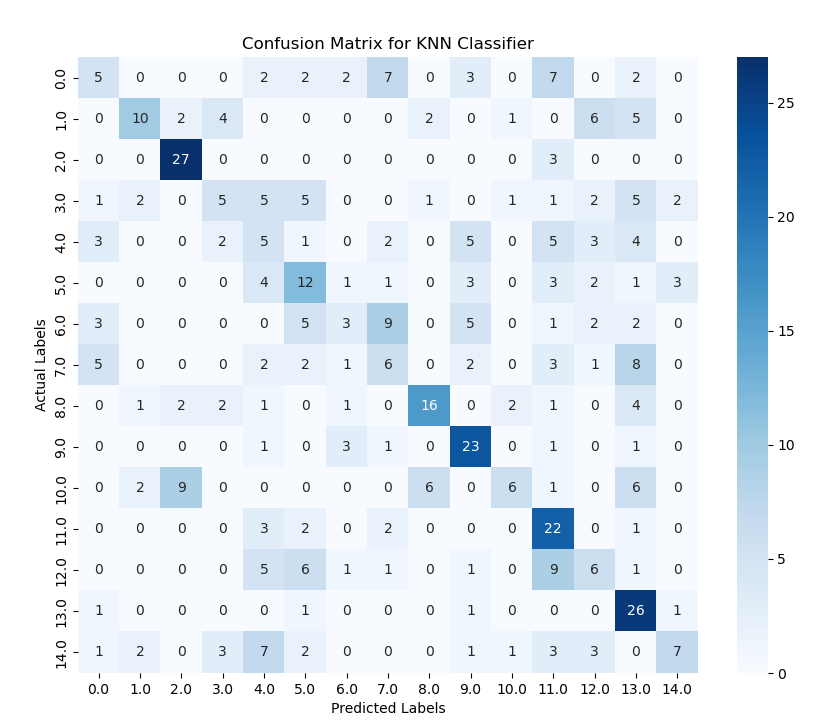
\includegraphics[width=0.8\textwidth]{imgs/knn.png} 
\end{center}

\subsection*{Choosing Regularization for SVM}

Choosing a $C=25$ improves the performance to around $49\%$ accuracy. The improvement is due to the regularization of the SVM model which helps to prevent overfitting to the training data.

\begin{center}
  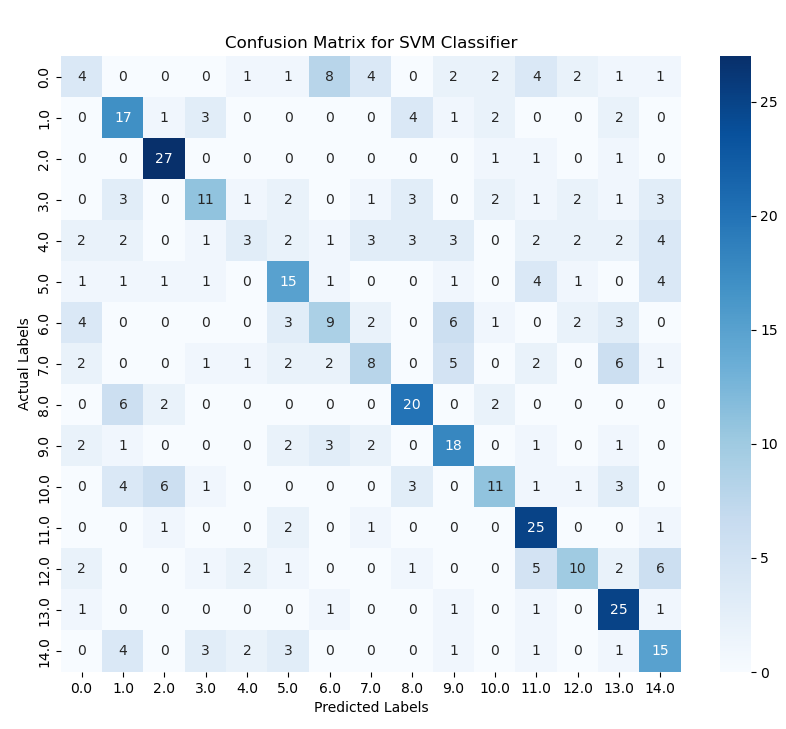
\includegraphics[width=0.8\textwidth]{imgs/svm.png} 
\end{center}

Overall it is great that the models can improve over random guessing when it comes to classification but an accuracy of only $50\%$ is not very good. The models both have removed important spatial distribution information that could help with classification. In addition the models are ultimatelt linear in nature with some primitive human engineered features when it comes to descriptors. The SIFT descriptors are good for finding unique points and mapping them across images or frames but they are not very good at describing the overall image.

\end{document}